\documentclass[compress]{beamer}
\usetheme{sthlm}

%-=-=-=-=-=-=-=-=-=-=-=-=-=-=-=-=-=-=-=-=-=-=-=-=
%        LOADING BEAMER PACKAGES
%-=-=-=-=-=-=-=-=-=-=-=-=-=-=-=-=-=-=-=-=-=-=-=-=

\usepackage{
booktabs,
datetime,
dtk-logos,
graphicx,
multicol,
pgfplots,
ragged2e,
tabularx,
tikz,
wasysym,
multirow,
float,
caption,
subcaption
}

\pgfplotsset{compat=1.8}

\usepackage[utf8]{inputenc}
\usepackage[portuguese]{babel}
\usepackage[T1]{fontenc}
\usepackage{newpxtext,newpxmath}
\usepackage{listings}

\lstset{ %
language=[LaTeX]TeX,
basicstyle=\normalsize\ttfamily,
keywordstyle=,
numbers=left,
numberstyle=\tiny\ttfamily,
stepnumber=1,
showspaces=false,
showstringspaces=false,
showtabs=false,
breaklines=true,
frame=tb,
framerule=0.5pt,
tabsize=4,
framexleftmargin=0.5em,
framexrightmargin=0.5em,
xleftmargin=0.5em,
xrightmargin=0.5em
}



%-=-=-=-=-=-=-=-=-=-=-=-=-=-=-=-=-=-=-=-=-=-=-=-=
%        LOADING TIKZ LIBRARIES
%-=-=-=-=-=-=-=-=-=-=-=-=-=-=-=-=-=-=-=-=-=-=-=-=

\usetikzlibrary{
backgrounds,
mindmap
}

%-=-=-=-=-=-=-=-=-=-=-=-=-=-=-=-=-=-=-=-=-=-=-=-=
%        BEAMER OPTIONS
%-=-=-=-=-=-=-=-=-=-=-=-=-=-=-=-=-=-=-=-=-=-=-=-=

\setbeameroption{show notes}

%-=-=-=-=-=-=-=-=-=-=-=-=-=-=-=-=-=-=-=-=-=-=-=-=
%        BEAMER COMMANDS
%-=-=-=-=-=-=-=-=-=-=-=-=-=-=-=-=-=-=-=-=-=-=-=-=


%-=-=-=-=-=-=-=-=-=-=-=-=-=-=-=-=-=-=-=-=-=-=-=-=
%
%	PRESENTATION INFORMATION
%
%-=-=-=-=-=-=-=-=-=-=-=-=-=-=-=-=-=-=-=-=-=-=-=-=

\title{Gerenciamento de \\ replicações}
\subtitle{DCE540 - Computação Paralela e Distribuída}
%\date{\small{\jobname}}
\author{\texttt{Iago Carvalho}}
\institute{\texttt{Departamento de Ciência da Computação}}

\hypersetup{
pdfauthor = {Iago A. Carvalho},      
pdfsubject = {Computação Paralela e Distribuída},
pdfkeywords = {},  
pdfmoddate= {D:\pdfdate},          
pdfcreator = {WriteLaTeX}
}

\begin{document}

\begin{frame}
\titlepage

\end{frame}

%% --------------------------------------------------------

\begin{frame}{Como, quando e onde replicar}

Dois problemas devem ser resolvidos na tomada de decisão da replicação
\begin{enumerate}
    \item Onde os servidores de réplicas estão localizados
    \item Onde os dados replicados estão localizados
\end{enumerate}

\vspace{0.5cm}

O primeiro tem como objetivo estabelecer o local físico (ou geográfico) dos servidores

\vspace{0.5cm}

O segundo diz respeito a qual dado será replicado em cada um dos servidores

\end{frame}

%% --------------------------------------------------------

\begin{frame}{Localização do servidor}

Este era um problema grave a alguns anos atrás

\vspace{0.5cm}

Entretanto, com o avanço da velocidade (e estabilidade) das conexões, isto deixou de ser um problema

\vspace{0.5cm}

Atualmente, existem heurísticas capazes de computar boas localizações para servidores em questão de segundos
\begin{itemize}
    \item O problema pode ser resolvido praticamente em tempo real
\end{itemize}

\end{frame}

%% --------------------------------------------------------

\begin{frame}{Replicação de conteúdo e localização}

\vspace{0.7cm}

\centering 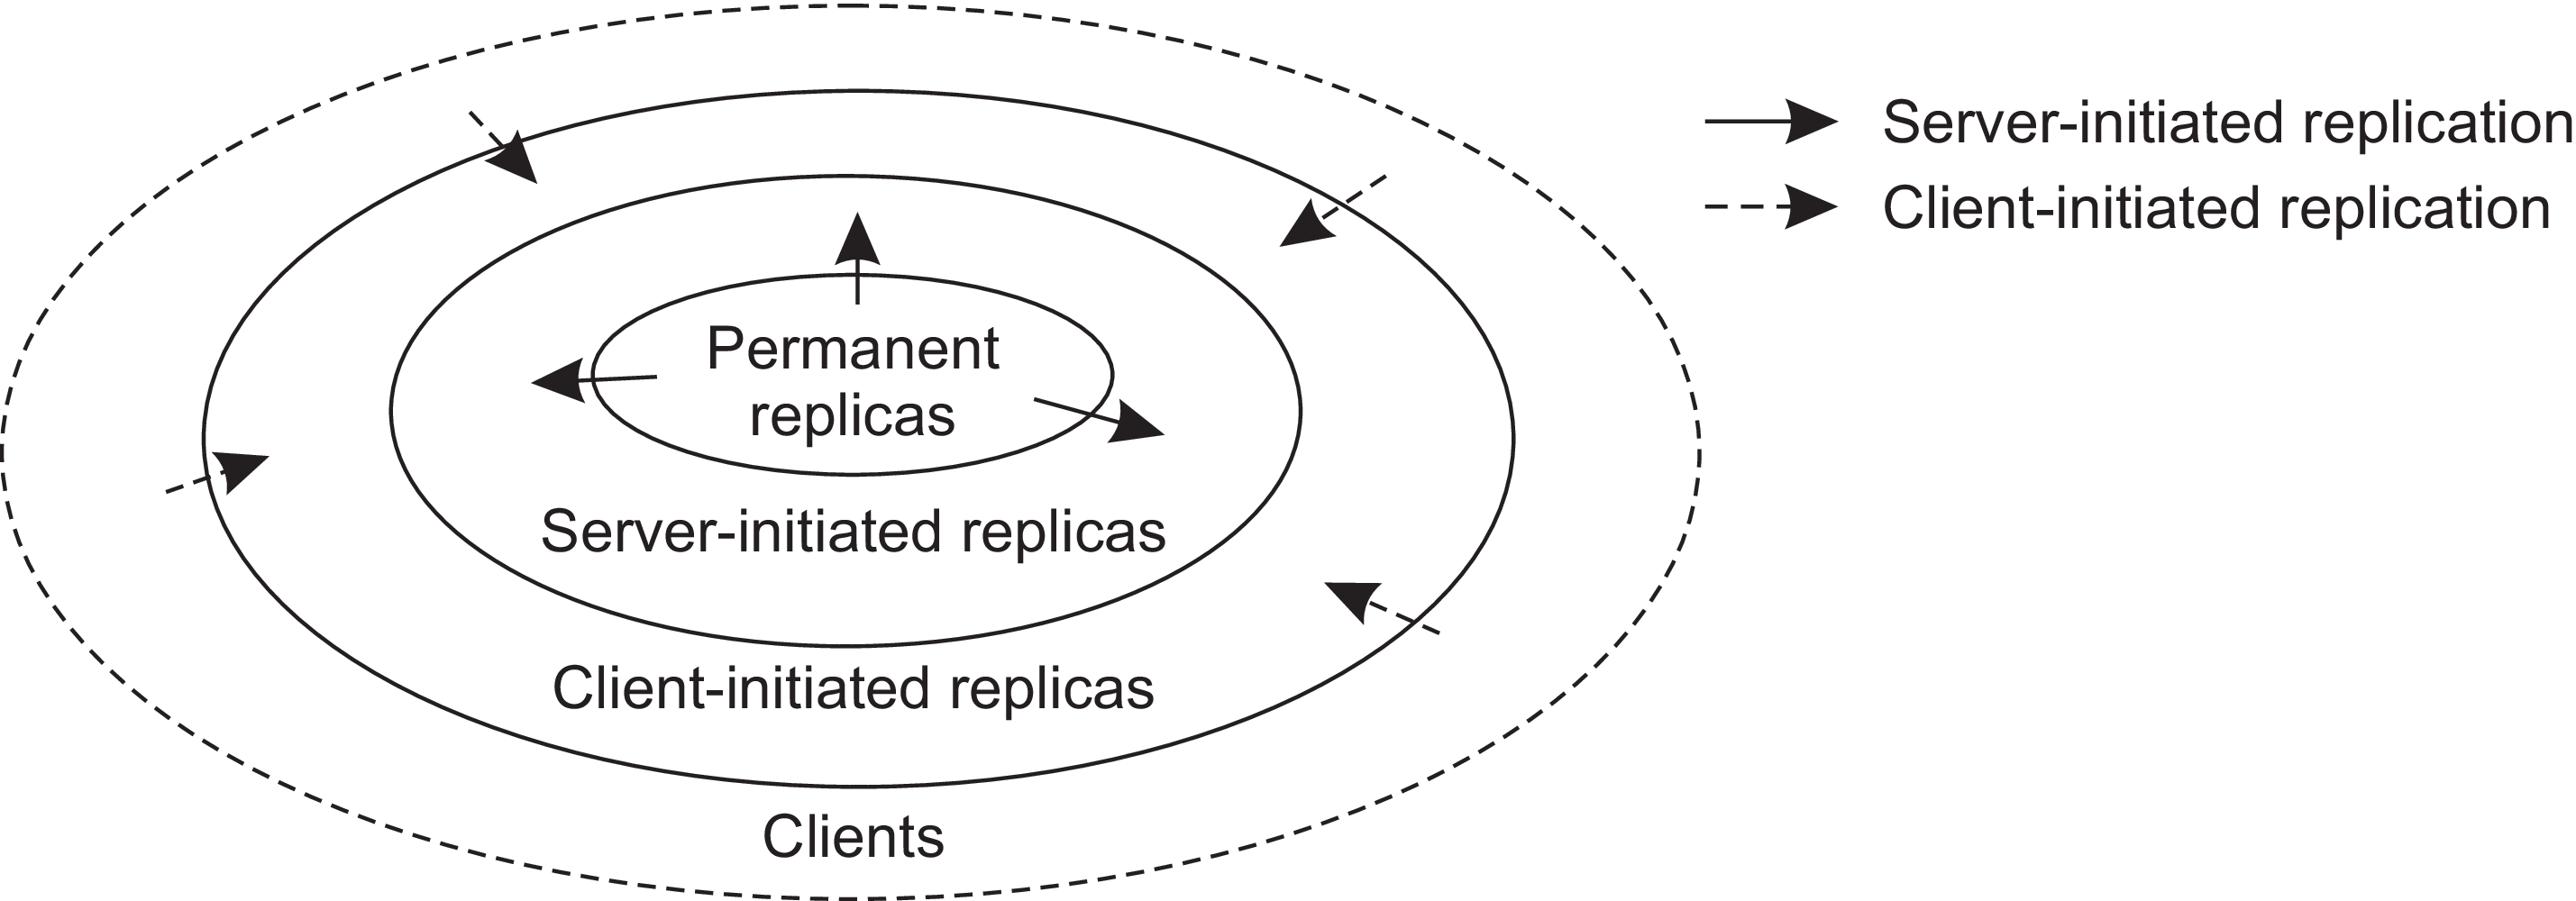
\includegraphics[width=\textwidth]{images/replicas.png}

\end{frame}

%% --------------------------------------------------------

\begin{frame}{Réplicas permanentes}

Estas são as réplicas iniciais do sistema distribuído
\begin{itemize}
    \item Normalmente é um pequeno conjunto 
    \item Estas réplicas são permanentes e nunca são removidas
\end{itemize}

\vspace{0.5cm}

Representa a cópia original dos dados
\begin{itemize}
    \item Seus espelhos através da internet
\end{itemize}
\end{frame}

%% --------------------------------------------------------

\begin{frame}{Réplicas iniciadas pelos servidores}

Muito comum hoje em dia com ambiente em nuvem e DevOps

\vspace{0.5cm}

Um servidor pode criar um número de réplicas adicionais para suportar um grande número de requisições
\begin{itemize}
    \item Estas réplicas normalmente são temporárias
    \item Réplicas são \textit{read-only}
\end{itemize}

\vspace{0.5cm}

Esta estratégia muitas vezes é utilizada quando ocorrem eventos específicos
\begin{itemize}
    \item Por exemplo, venda de ingressos para festivais
\end{itemize}
\end{frame}

%% --------------------------------------------------------

\begin{frame}{Réplicas iniciadas pelos clientes}

Este tipo de replicação de dados não pode ser controlado pelo sistema distribuído

\vspace{0.5cm}

Uma réplica iniciada pelo cliente é um dado (ou conjunto de dados) \textit{cache}
\begin{itemize}
    \item Localizado na própria máquina do cliente ou em algum dispositivo de rede muito próximo a ele
    \item Muito útil quando o cliente faz diversas requisições a um mesmo conjunto de dados
\end{itemize}

\vspace{0.5cm}

Este tipo de réplica tem um tempo de vida limitado e é de responsabilidade do cliente atualizar seus dados
\end{frame}

%% --------------------------------------------------------

\begin{frame}{Distribuição de dados}

A primeira coisa a se preocupar é com quais dados propagar

\vspace{0.5cm}

No geral, existem três opções
\begin{enumerate}
    \item Propagar uma notificação da atualização dos dados 
    \begin{itemize}
        \item Protocolo de invalidação
    \end{itemize}
    \item Propagar o dado alterado (por completo)
    \item Propagar somente a alteração que o dado sofreu \begin{itemize}
        \item Replicação ativa
    \end{itemize}
\end{enumerate}

\end{frame}

%% --------------------------------------------------------

\begin{frame}{\textit{Push} ou \textit{pull}}

Os updates serão enviados pelo servidor ou serão requisitados pelos clientes?

\vspace{0.25cm}

Esquema baseado em \textit{push}
\begin{itemize}
    \item Os dados são replicados a partir do servidor
    \item Utilizado quando deseja-se manter uma consistência apertada
    \item Útil quando a maioria das operações dos clientes são de leitura
    \item Maior custo de rede
\end{itemize}

\vspace{0.25cm}

Esquema baseado em \textit{pull}
\begin{itemize}
    \item Clientes tem que requisitar a atualização dos dados
    \item Útil junto com protocolos de invalidação
    \item Tempo de resposta relativamente alto
    \begin{itemize}
        \item Pode ser necessário atualizar os dados ao fazer uma requisição
    \end{itemize}
\end{itemize}
\end{frame}

%% --------------------------------------------------------

\begin{frame}{\textit{Unicast} ou \textit{multicast}}

Como transferir os dados?

\vspace{0.5cm}

\textit{Unicast}
\begin{itemize}
    \item Atualização é realizada em uma comunicação direta entre dois dispositivos
    \item Necessárias $N$ mensagens para atualizar todo o sistema distribuído
    \item Útil no caso de esquema de atualização baseado em \textit{pull}
\end{itemize}

\vspace{0.5cm}

\textit{Multicast}
\begin{itemize}
    \item Atualização é realizada de um dispositivo para diversos outros
    \item Um único processo de comunicação é necessário para atualizar quantos servidores forem necessários
    \item Útil no caso de esquema de atualização baseado em \textit{push}
\end{itemize}
\end{frame}

\end{document}
